\begin{center}
    \begin{figure}[H]
        \centering

        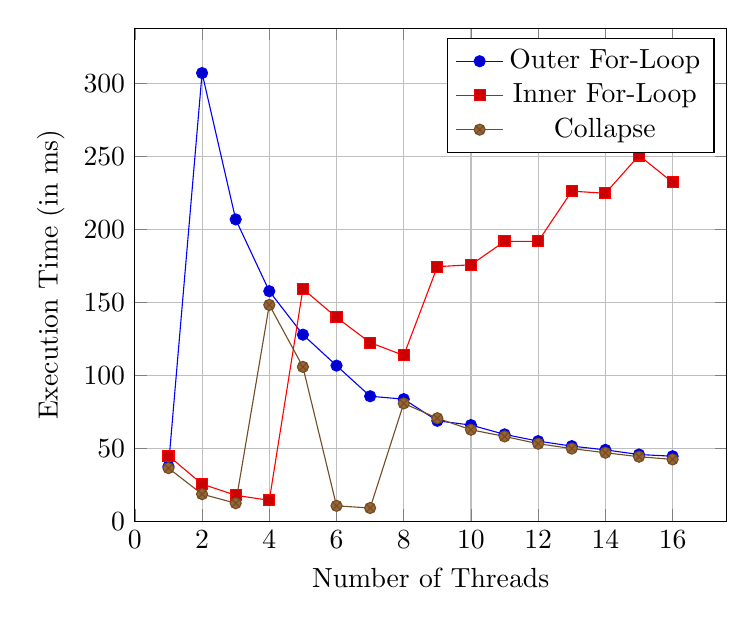
\begin{tikzpicture}
            \begin{axis}[
                title={},
                width=0.75\textwidth,
                xlabel={Number of Threads},
                ylabel={Execution Time (in ms)},
                xmin=0,
                ymin=0,
                grid=major
            ]
                \addplot coordinates {
                    (1,37.6298)(2,307.277)(3,206.951)(4,157.739)(5,127.945)(6,106.722)(7,85.7366)(8,83.7447)(9,68.8881)(10,65.9673)(11,59.5942)(12,54.9606)(13,51.537)(14,48.9599)(15,45.7805)(16,44.6108)
                };
                \addlegendentry{Outer For-Loop}

                \addplot coordinates {
                    (1,44.9149)(2,25.5319)(3,17.8099)(4,14.3929)(5,159.317)(6,139.78)(7,122.484)(8,113.725)(9,174.565)(10,175.844)(11,191.872)(12,191.879)(13,226.324)(14,224.853)(15,250.807)(16,232.331)
                };
                \addlegendentry{Inner For-Loop}       

                \addplot coordinates {
                    (1,36.462)(2,18.6164)(3,12.3985)(4,148.35)(5,105.857)(6,10.613)(7,9.119)(8,80.8353)(9,70.6663)(10,62.7591)(11,58.1758)(12,53.1777)(13,49.8448)(14,46.9922)(15,44.2674)(16,42.432)
                };
                \addlegendentry{Collapse}
            \end{axis}
        \end{tikzpicture}
        \caption{Emboss Performance Tests dice.png}
    \end{figure}
\end{center}